\documentclass[onecolumn]{article}
\usepackage{graphicx}
\usepackage{float}
\usepackage{hyperref}
\restylefloat{figure}
\begin{document}

\title{Sums of squares -- how many possibilities?}

\author{Arjen Markus}

\maketitle

\section*{Introduction}
It is well-known that any positive integer can be written as the sum of at most four squares, a fact that is known as \emph{Lagrange's four square theorem}.\footnote{\url{https://mathworld.wolfram.com/LagrangesFour-SquareTheorem.html}}
For instance:
\begin{eqnarray*}
     7 &=& 2^2 + 1^2 + 1^2 + 1^2 \\
    10 &=& 3^2 + 1^2 \\
    15 &=& 3^2 + 2^2 + 1^2 + 1^2
\end{eqnarray*}

Many integers can be written as such a sum in different ways:
\begin{eqnarray*}
    10 &=& 3^2 + 1^2 \\
       &=& 2^2 + 2^2 + 1^2 + 1^2 \\
    50 &=& 7^2 + 1^2 \\
       &=& 5^2 + 5^2 \\
       &=& 6^2 + 3^2 + 2^2 + 1^2
\end{eqnarray*}

Let us be precise: if we ignore the order of the terms and allow only positive integers, then the following, somewhat lengthy program will print the
sequences of up to four squares that add up to a given number:

\begin{verbatim}
program explicit_loops
    implicit none

    character(len=20) :: string
    integer           :: number, maxi, maxj, maxk, maxl, count
    integer           :: i, j, k, l

    if ( command_argument_count() < 1 ) then
        write( *, * ) 'What is the number?'
        read( *, * )  number
    else
        call get_command_argument( 1, string )
        read( string, * ) number
    endif

    write( *, * ) 'Number to be written as a sum of squares:', number

    maxl = isqrt(number)  ! Make sure we have the largest possible integer

    count = 0
    do l = maxl,1,-1

        if ( l**2 == number ) then
            count = count + 1
            write(*,*) count, ':', l
            cycle
        endif

        maxk = isqrt(l**2)
        do k = maxk,1,-1

            if ( l**2 + k**2 == number ) then
                count = count + 1
                write(*,*) count, ':', l, k
                cycle
            endif

            maxj = isqrt(k**2)
            do j = maxj,1,-1

                if ( l**2 + k**2 + j**2 == number ) then
                    count = count + 1
                    write(*,*) count, ':', l, k, j
                    cycle
                endif

                maxi = isqrt(j**2)
                do i = maxi,1,-1

                    if ( l**2 + k**2 + j**2 + i**2 == number ) then
                        count = count + 1
                        write(*,*) count, ':', l, k, j, i
                    endif
                enddo
            enddo
        enddo
    enddo

    write(*,*) 'Total number of solutions: ', count
contains

integer function isqrt( n )
    integer, intent(in) :: n

    isqrt = int( sqrt(real(n)) )

    !
    ! Take care of possible rounding errors (if n is very large)
    !
    if ( (isqrt+1)**2 == n ) then
        isqrt = isqrt + 1
    endif
end function isqrt

end program explicit_loops
\end{verbatim}

(Note that for large integers, determining the largest square that is equal or smaller than the given integer via \verb+int( sqrt( real(n) ) )+ may produce
too small a value, due to truncation. The function \verb+isqrt+ is meant to prevent that from happening.)

It works as follows:
\begin{itemize}
\item
Given a number $n$, determine the largest integer $l$ such that $l^2 \leq n$. This is the start of the first loop. All other integers to be squared
should be equal or lower than the index of the first loop.
\item
The difference $n - l^2$ determines the start of the second loop: $k^2 \leq (n - l^2)$ and so on.
\item
Print the result if the sum is equal to the given number $n$.
\end{itemize}

\begin{table}
\begin{center}
\caption{Number of solutions (N) for a few integers (n).}
\label{uptofour}
\begin{tabular}{rr|rr|rr}
\emph{n} & \emph{N} & \emph{n} & \emph{N} & \emph{n} & \emph{N} \\
\hline
    1    &    1     &   11     &     1    &   30     &     2    \\
    2    &    1     &   12     &     2    &   40     &     2    \\
    3    &    1     &   13     &     2    &   50     &     5    \\
    4    &    2     &   14     &     1    &   60     &     3    \\
    5    &    1     &   15     &     1    &   70     &     5    \\
    6    &    1     &   16     &     2    &   80     &     2    \\
    7    &    1     &   17     &     2    &   90     &     9    \\
    8    &    1     &   18     &     3    &   100    &     7    \\
    9    &    2     &   19     &     2    &   200    &     5    \\
   10    &    2     &   20     &     2    &   300    &    13    \\
\hline
\end{tabular}
\end{center}
\end{table}

It will produce a list of all the combinations, as required (see Table \ref{uptofour} for several values of $n$).

\section{Recursive solution}
The code of the program in the previous section is repetitive as
the four integers are each determined in their own loop and therefore it would be tedious to extend it to, say, the sum of cubes -- every integer can
be written as the sum of at most nine cubes or 19 fourth-powers.\footnote{\url{https://en.wikipedia.org/wiki/Waring\%27s\_problem}}. So, let's
look at an alternative, using recursion:

\begin{verbatim}
program recursive_solution
    implicit none

    character(len=20) :: string
    integer           :: number, maxvalue, count
    integer           :: values(0)

    ... as in the first program

    write( *, * ) 'Number to be written as a sum of squares:', number

    maxvalue = isqrt(number)  ! Make sure we have the largest possible integer

    count = 0
    call determine_solutions( number, maxvalue, count, values )

    write(*,*) 'Total number of solutions: ', count
contains

recursive subroutine determine_solutions( number, maxvalue, count, values )
    integer, intent(in)    :: number
    integer, intent(in)    :: maxvalue
    integer, intent(inout) :: count
    integer, intent(in)    :: values(:)

    integer                :: i
    integer                :: maxnext

    do i = maxvalue,1,-1

        if ( size(values) < 4 ) then
            if ( number == i**2 ) then
                count = count + 1
                write(*,*) count, ':', [values, i]

            elseif ( number > i**2 ) then
                maxnext = isqrt(i**2)
                call determine_solutions( number-i**2, maxnext, count, [values, i] )
            endif
        endif
    enddo
end subroutine determine_solutions

... function isqrt is the same

end program recursive_solution
\end{verbatim}

This program works in much the same way but instead of a nested do-loop, it calls itself with
adjusted arguments. One of these arguments is the list of integers that should add up to the
given number $n$. But it only does so if the list is short enough: we want four integers, no more.

\section{Sums of more than four squares}

The recursive construction allows us to easily vary the program so that other mathematical problems
can be solved:
\begin{itemize}
\item
How can a number be written as at most nine cubes?
\item
What if you allow any number of squares?
\end{itemize}

To illustrate the latter mathematical problem, the number 10 can be written as:
\begin{eqnarray*}
    10 &=& 3^2 + 1^2 \\
       &=& 2^2 + 2^2 + 1^2 + 1^2 \\
       &=& 2^2 + 1^2 + ... + 1^2 \\
       &=& 1^2 + ... + 1^2
\end{eqnarray*}

\begin{figure}[H]
\caption{Number of solutions for the sum of any number of squares equal to the given value. See text for further information.}
\label{unlimitedgraph}
\begin{center}
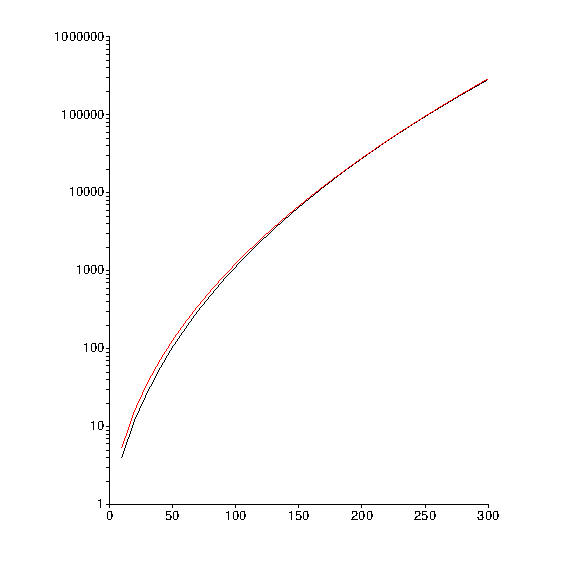
\includegraphics[width=0.9\textwidth]{number_solutions.pdf}
\end{center}
\end{figure}

Table \ref{unlimitedsum} shows the number of solutions for a few values of $n$. As can be seen, the number
grows very fast (see also Figure \ref{unlimitedgraph}). The red line in the figure was estimated visually, the
number of solutions is approximately, at least up to $n = 300$:

\begin{eqnarray*}
    N(n) &\approx& 0.5~ e^{n^{0.46}}
\end{eqnarray*}

\begin{table}
\begin{center}
\caption{Number of solutions (N) for the sum of any number of squares for a few integers (n).}
\label{unlimitedsum}
\begin{tabular}{rr|rr|rr}
\emph{n} & \emph{N}         & \emph{n} & \emph{N}    & \emph{n}    & \emph{N}    \\
\hline
10       &         4        & 110      &    1653     &    210      &  35750      \\
20       &         12       & 120      &    2374     &    220      &  46030      \\
30       &         27       & 130      &    3385     &    230      &  59027      \\
40       &         55       & 140      &    4714     &    240      &  75005      \\
50       &         104      & 150      &    6521     &    250      &  94987      \\
60       &         178      & 160      &    8849     &    260      &  119360     \\
70       &         302      & 170      &    11953    &    270      &  149482     \\
80       &         476      & 180      &    15895    &    280      &  185960     \\
90       &         747      & 190      &    21031    &    290      &  230580     \\
100      &         1116     & 200      &    27482    &    300      &  284316     \\
\hline
\end{tabular}
\end{center}
\end{table}

This mathematical problem also leads to an interesting programming problem: with the recursive
solution we consume more and more memory and at some point (for $n$ large enough), the stack memory
is exhausted. Experimentation shows that this happens around $n = 3000$ (simply set the variable
\verb+maxvalue+ to 1 or 2 instead of \verb+isqrt(n)+ and enter a largish number) -- the program dies
without printing the number of solutions.

The amount of memory taken from the stack for each recursion can be limited either by compile options
(to take the required memory for the constructed array from the heap) or by using a fixed array and counting
the number of integers separately. A more interesting solution is to combine iteration and recursion.

\begin{verbatim}
program iterative_unlimited
    implicit none

    character(len=20)    :: string
    integer              :: idx, number, maxvalue, count, residue
    integer, allocatable :: values(:)

    ... same as the other programs

    write( *, * ) 'Number to be written as a sum of squares:', number

    allocate( values(number) ) ! Provide the storage

    count = 0
    idx   = 1

    values    = 0
    values(1) = maxvalue

    do
        residue  = number - sum(values(1:idx)**2)

        if  ( residue > 0 ) then
            maxvalue = min( isqrt(residue), values(idx) )

            if ( maxvalue > 0 ) then
                idx = idx + 1
                values(idx) = maxvalue
            endif

        elseif ( residue == 0 ) then
            count = count + 1
            write(*,*) count, ':', values(1:idx)

            do while ( values(idx) > 0 )
                values(idx) = values(idx) - 1

                if ( values(idx) <= 0 ) then
                    idx = idx - 1
                else
                    exit
                endif
            enddo

        else
            if ( values(idx) > 1 ) then
                values(idx) = values(idx) - 1
            else
                idx = idx - 1
            endif
        endif

        if ( idx <= 0 ) then
            exit
        endif
    enddo

    write(*,*) 'Total number of solutions: ', count
contains
...
end program iterative_unlimited
\end{verbatim}

The program uses a fixed amount of memory and uses a work array \verb+values+ to keep track of the solution
and the candidates. Via the indeterminate loop together with the index \verb+idx+ by which the work array is
adjusted, the program iterates over all sets of integers ${v_i}$ such that the following conditions hold:
\begin{eqnarray*}
     v_{i+1}      &\leq& v_i  ~~~~~~~~i < n \\
     \Sigma v_i^2 &\leq& n
\end{eqnarray*}

Note that this means that if $v_i$ becomes zero, the index $i$ has to be decreased.

The logic is more complicated, but it is now (in principle) possible to determine the number of solutions for
very large values of $n$.

\end{document}
